%=================================================================

\section{Introduction}\label{sec-intro}

\subsection{Problem Statement}


After a month of making scientific observations 
and taking careful measurements, 
can determined that 900 ghouls, ghosts, and goblins
like what is shown in~\Cref{fig:animal}  .
The raw dataset contains train set with 10000 %modify as your true values
samples and 5000 unlabeled samples as test set.
Through the train data, I can find the relationship
between the attributes and species, and then identify 371 of the ghastly creatures.


\begin{figure}[htbp]
	\centering
	%\graphicspath{figures}
	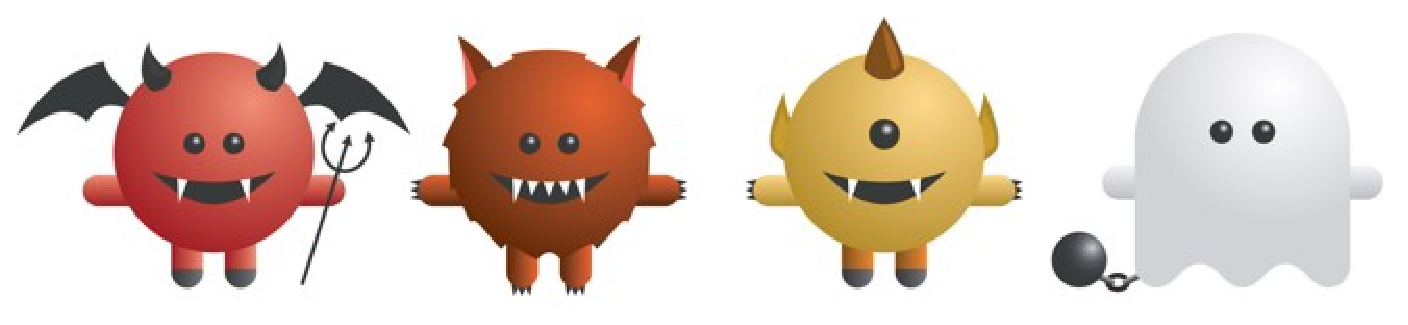
\includegraphics[scale=0.3]{figures/bar.eps}
	\caption{The Picture of Ghastly}\label{fig:animal}
\end{figure}


\subsection{Data List}


There are bone length measurements, 
severity of rot, extent of soullessness, 
and other characteristics of the intruders,
the fllowings are the  
name and meaning of attributes


\begin{description}
	\item[id] id of the creature
	\item[bone_length] average length of bone in the creature, normalized between 0 and 1
	\item[rotting_flesh] percentage of rotting flesh in the creature
	\item[hair_length] average hair length, normalized between 0 and 1
	\item[has_soul] percentage of soul in the creature
	\item[Color] dominant color of the creature: 'white','black','clear','blue','green','blood'
	\item[type] target variable: 'Ghost', 'Goblin', and 'Ghoul'
\end{description}


\subsection{Problem Analysis}

\subsubsection{Train Data and Test Data}


Because this game is over, 
it can't submit the predictive values for testing. 
So I divide the raw train set into train data and test data, 
and the ratio between the two is 8:2. 
Another vexed problem is the data too small, 
so I use ten-fold cross-validation 
to train the data.


\subsubsection{Problem Possible Solutions}


There are many machine learning algorithms 
can solve the three classification problem,
such as ensemble algorithms,
decision tree algorithm and so on.
Use CV to find the best parameters of the algorithms 
and then validate with testing data 


\subsubsection{Evaluation Methods}


Before experiment, determine the evaluation methods
to assess the model performance is very important,
usually it has two kinds of method for classification problem:

\begin{itemize}
	\item F1 Score/AUC
	\item Class Accuracy
\end{itemize} 


\section{Data exploration} \label{sec-data_exploration}

\subsection{Data Information}


The following table ~\cref{tbl:data information}
is the statistical result of the attribute values.
There are 4 numerical variables and 1 categorical. 
And no missing values.
Numerical columns are either normalized or show a percentage, 
so no need to scale them. 

\begin{table}[htbp]  \centering
	\caption{Data Information}
	\label{tbl:data information}
	\begin{tabular}{ccccccc}
		\hline
		% after \\: \hline or \cline{col1-col2} \cline{col3-col4} ...
		& bone_length & rotting_flesh & hair_length & has_soul & color & type\\
		\hline
		count & 371.0 & 371.0 & 371.0 & 371.0 & 371 & 371 \\
		unique & NaN & NaN & NaN & NaN & 6 & 3 \\
		top & NaN & NaN & NaN & NaN & white & Ghoul \\
		freq & NaN & NaN & NaN & NaN & 137 & 129\\
		mean & 0.434160 & 0.506848 & 0.529114 & 0.471392 & NaN & NaN \\
		std & 0.132833 & 0.146358 & 0.169902 & 0.176129 & NaN & NaN \\
		min & 0.061032 & 0.095687 & 0.134600 & 0.009402 & NaN & NaN \\
		25\% & 0.340006 & 0.414812 & 0.407428 & 0.348002 & NaN & NaN \\
		50\% & 0.43891 & 0.501552 & 0.538642 & 0.466372 & NaN & NaN\\
		75\% & 0.517223 & 0.603977 & 0.647244 & 0.600610 & NaN & NaN\\
		max &  0.817001 & 0.932466 & 1.000000 & 0.935721 & NaN & NaN\\
		\hline 
		%\bottomrule
	\end{tabular}
\end{table}


\subsection{Data Visualization}


Use EDA to plot the distribution of the data 
to can observate the data intuitively and
find the relation between the attribute values. 
For example boxplot can visually observe 
the distribution of numerical variables, 
scatterplot can show their distribution trends 
and whether there are outliers.
And for classification problems, 
the data is drawn according to 
the different colors of the Label, 
which is very helpful for 
the construction of the Feature.


\subsubsection{ Histogram}


The figure ~\Cref{fig:his_1} 
shows the mean of the four numerical variables  
and the figure ~\Cref{fig:his_2} 
is the number of different color 
about types of ghastly creatures.
It seems that all numerical features may be useful, 
but many colors are evenly distributes among the monsters. 
So they maybe not very useful for classification.


\begin{figure}[htbp]
	\centering
	
	%\graphicspath{{figures/}{mine/}}
	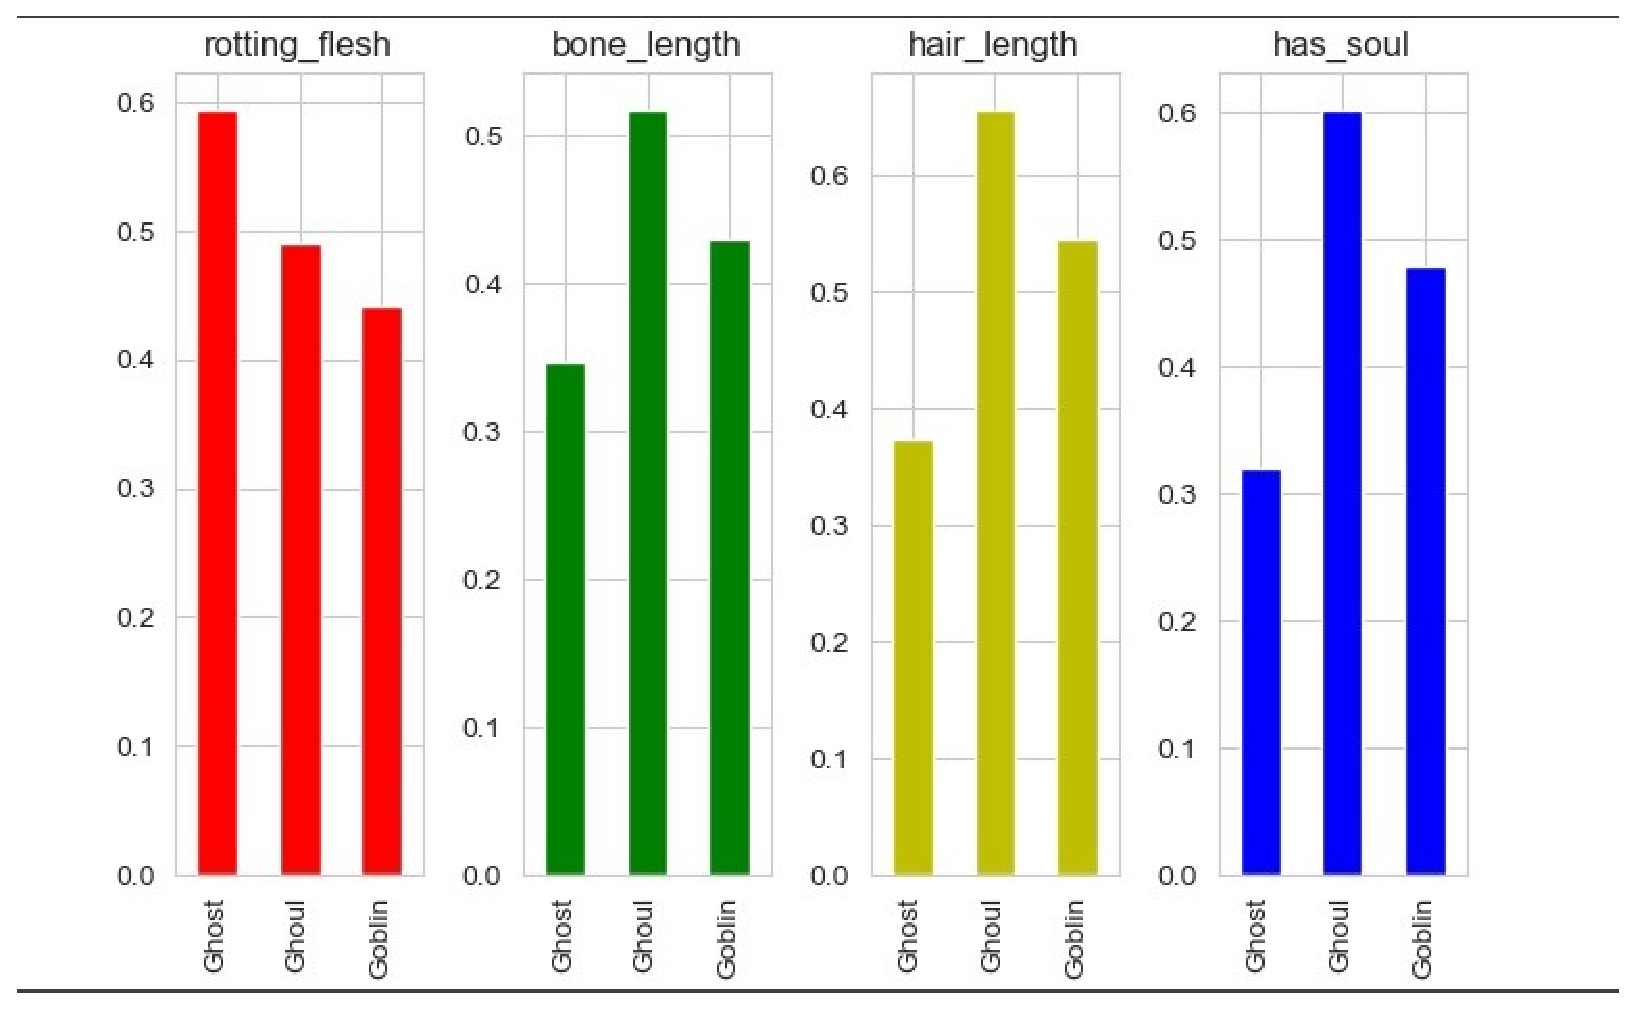
\includegraphics[scale=0.3]{figures/his_1.eps}
	\caption{The Mean of Four Numerical Variables}\label{fig:his_1}
\end{figure}


\begin{figure}[htbp]
	\centering
	
	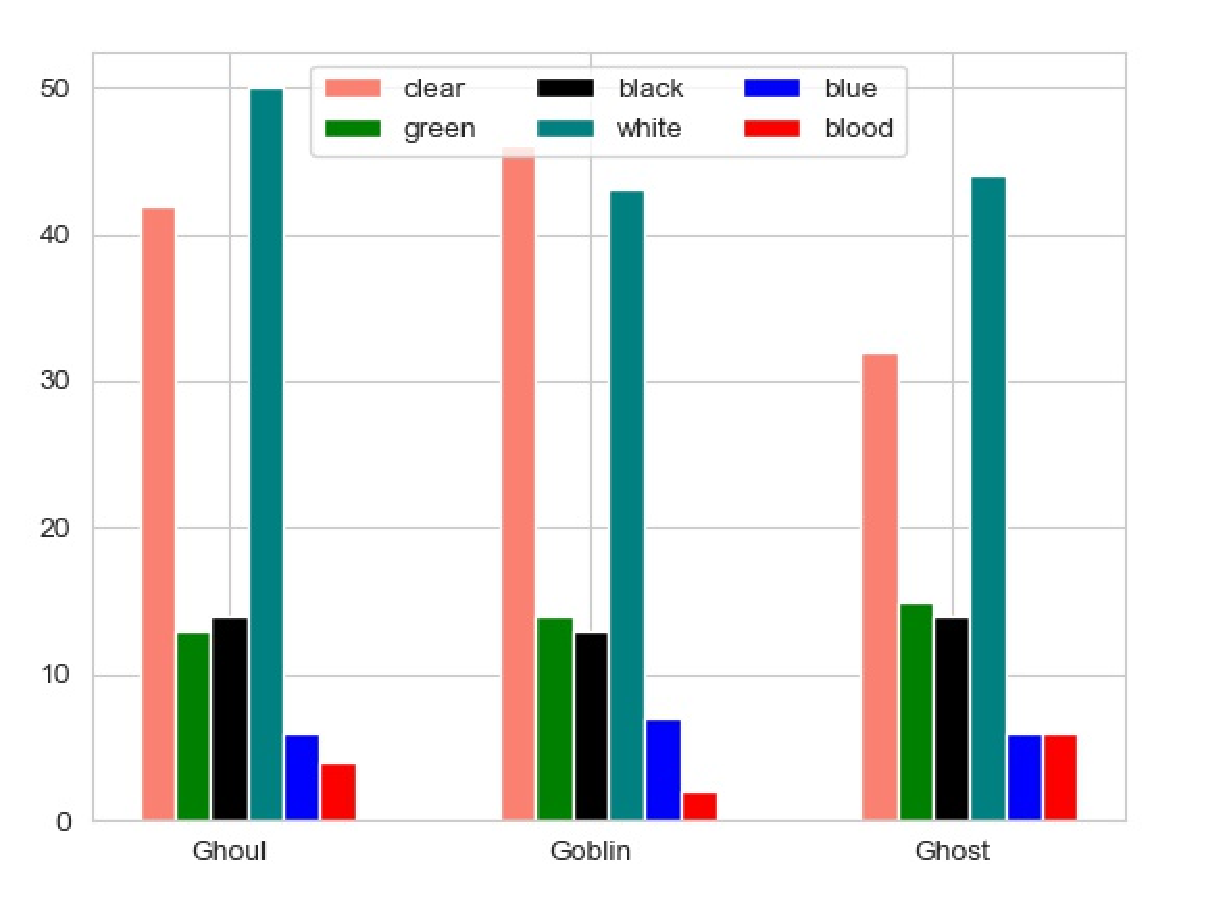
\includegraphics[scale=0.3]{figures/his_2.eps}
	\caption{Color distribution Grouped by Type}\label{fig:his_2}
\end{figure}


\subsubsection{Boxplot}

 
When analyzing the data, 
the boxplot can effectively 
help us identify the characteristics of the data: 
visually identify outliers in the dataset. 
Determine the data dispersion and 
bias of the data set. 
Through the figure ~\Cref{fig:boxplot}, 
know that the two types of Ghost and Ghoul 
in the monster have higher discrimination 
on the four variables, 
while Goblin is in the middle position, 
which intersects with the other two types of features.
Guess that the predictive accuracy of Ghost and Ghoul 
will be better than Goblin.
And the outliers are very small,
which can be ignored.


\begin{figure}[htbp]
	\centering
	
	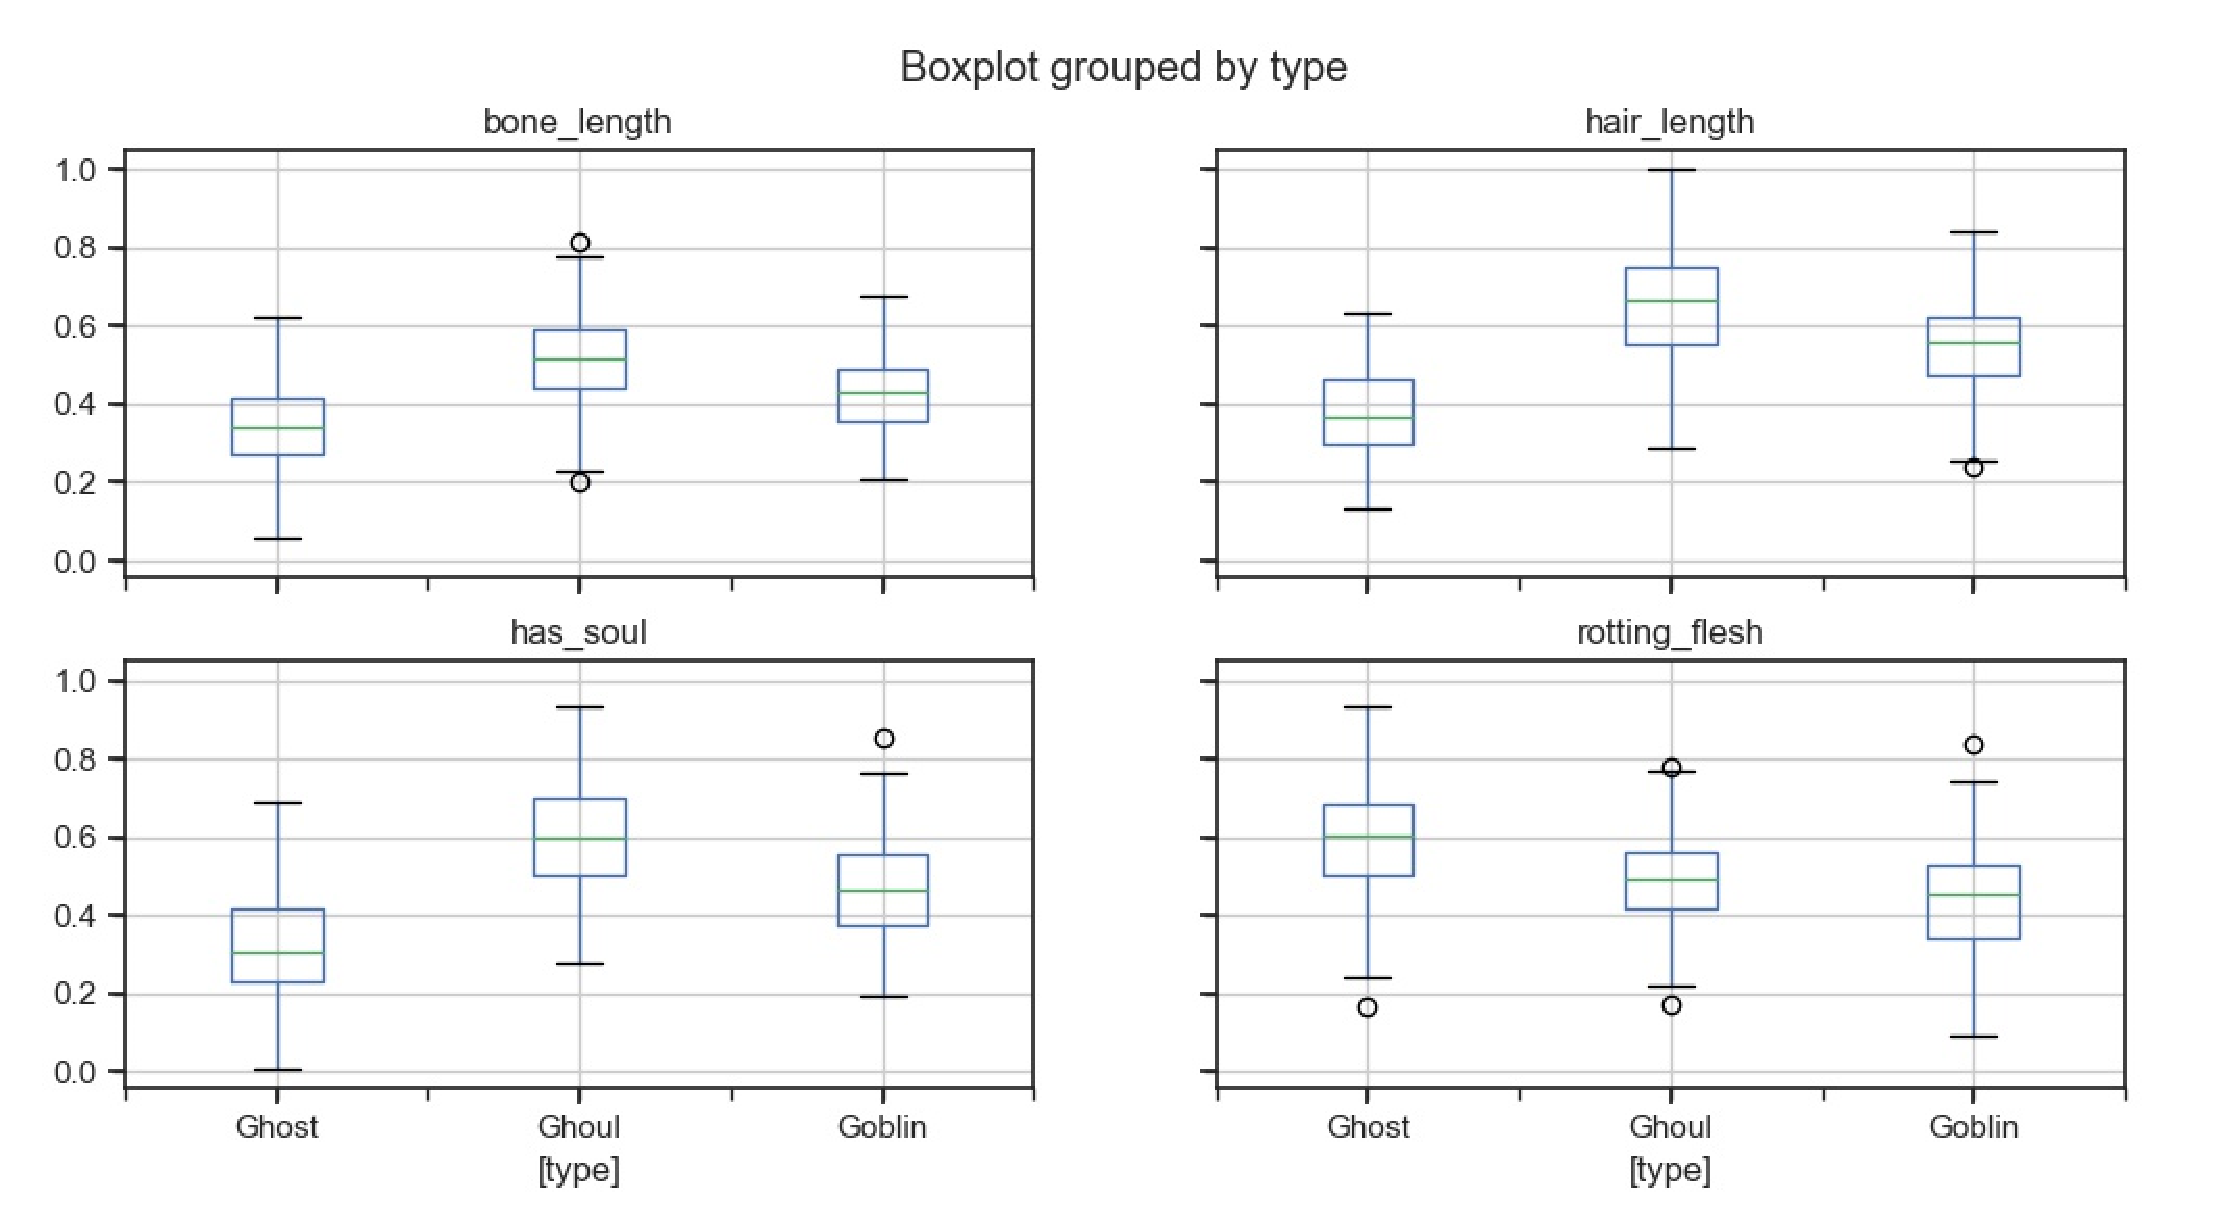
\includegraphics[scale=0.3]{figures/boxplot.eps}
	\caption{Boxplot Grouped by Type}\label{fig:boxplot}
\end{figure}


\subsubsection{Pairwise Plot} 


Pairwise plot is 
a favorite in exploratory analysis 
to understand the relationship 
between all possible pairs 
of numeric variables. 
This pairplot ~\Cref{fig:feature_scatterplot} 
shows that data is distributed normally. 
And while most pairs are widely scattered 
(in relationship to the type), 
some of them show clusters: 
hair_length and has_soul, 
hair_length and bone_length. 
So it may need to reassemble the data.

\begin{figure}[htbp]
	\centering
	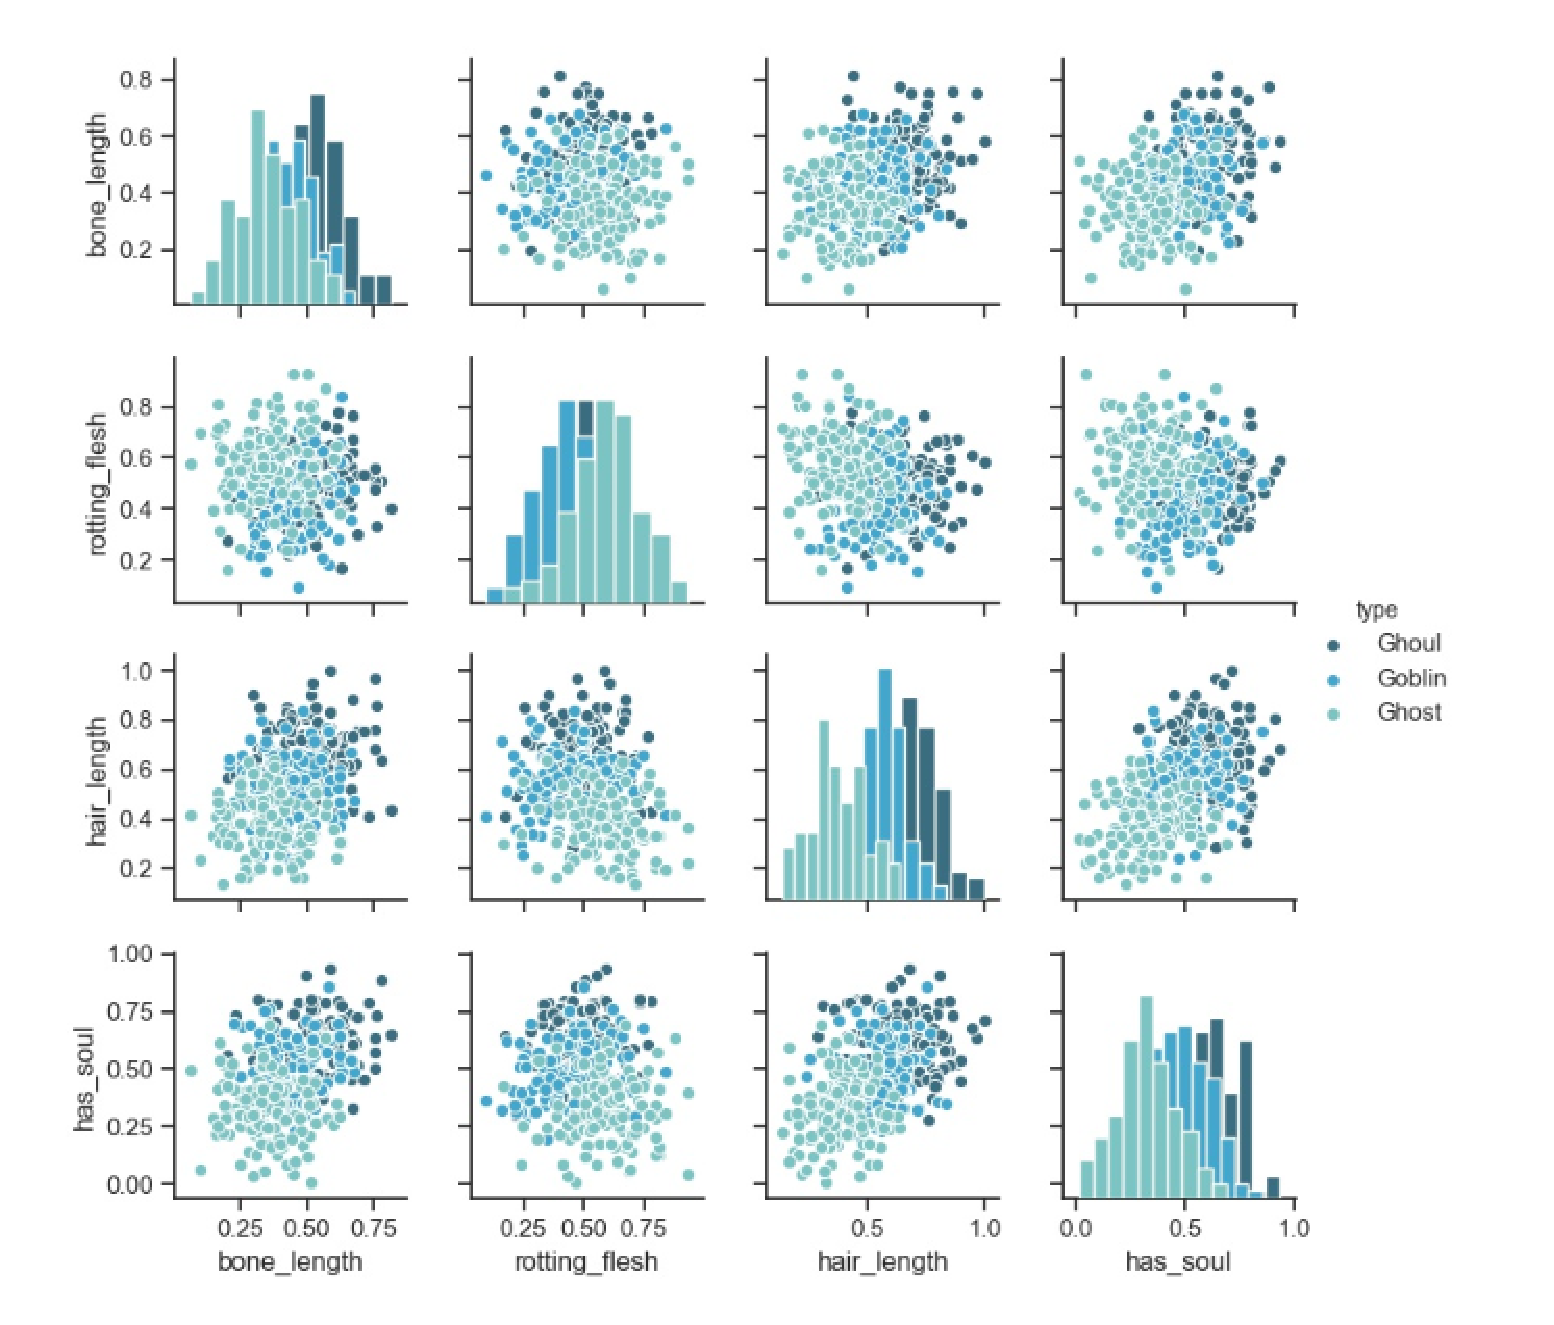
\includegraphics[scale=0.3]{figures/pairplot.eps}
	\caption{Feature Scatterplot}\label{fig:feature_scatterplot}
\end{figure}


\subsubsection{Correllogram}


Correlogram is used to 
visually see the correlation metric 
between all possible pairs of numeric variables 
in a given dataframe. 
This figure ~\Cref{fig:corr} 
help us to analyze features 
and their impact on the 'type' column. 
As we can see the 'type' column 
has a high value of negative correlation 
with columns 'has_soul' and 'rotting_flesh'. 
Although the correlation 
with the 'hair_length' is not very big.
There is no obvious linear relationship 
between variables

\begin{figure}[htbp]
	\centering
	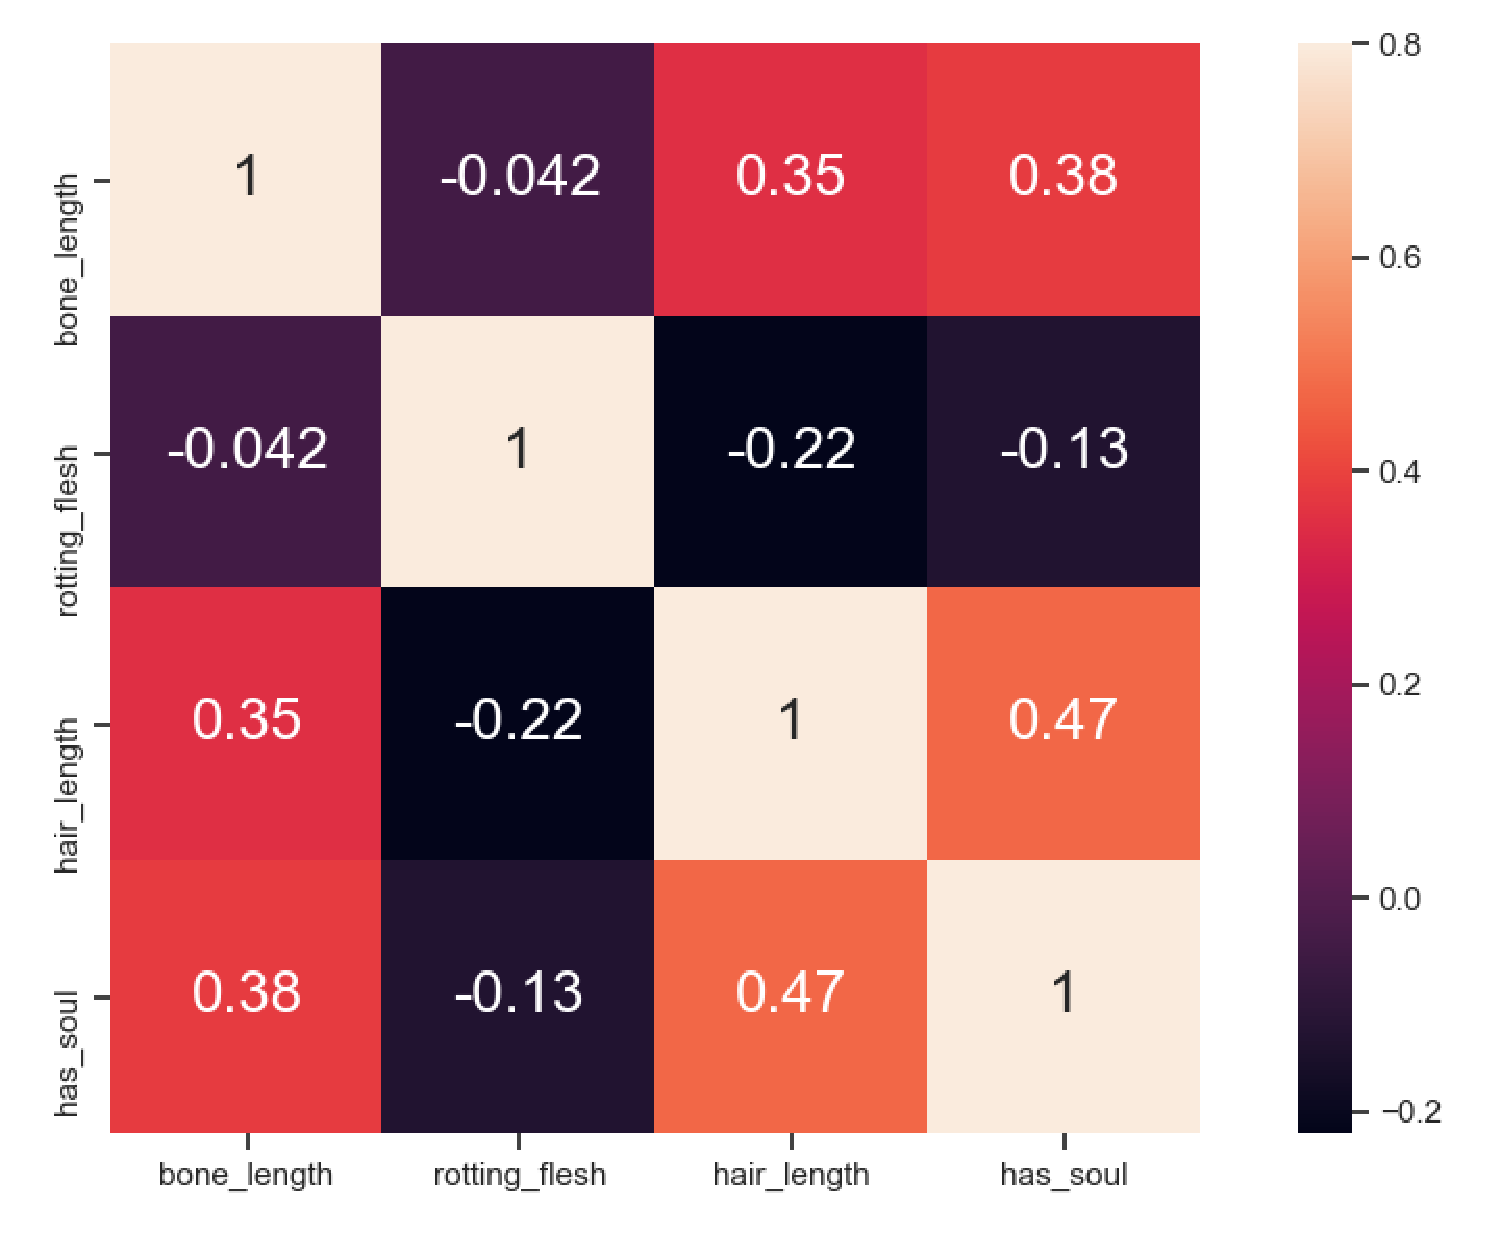
\includegraphics[scale=0.3]{figures/corr.eps}
	\caption{Correllogram}\label{fig:corr}
\end{figure}


\subsubsection{Other Figures}


The following pictures 
are independent of 
the choice of algorithm. 
Because they look great, 
so I want to share with you.
%如果有时间的话,把这三张图片放在一排,然后稍微介绍一下

\begin{figure}[h]\centering
	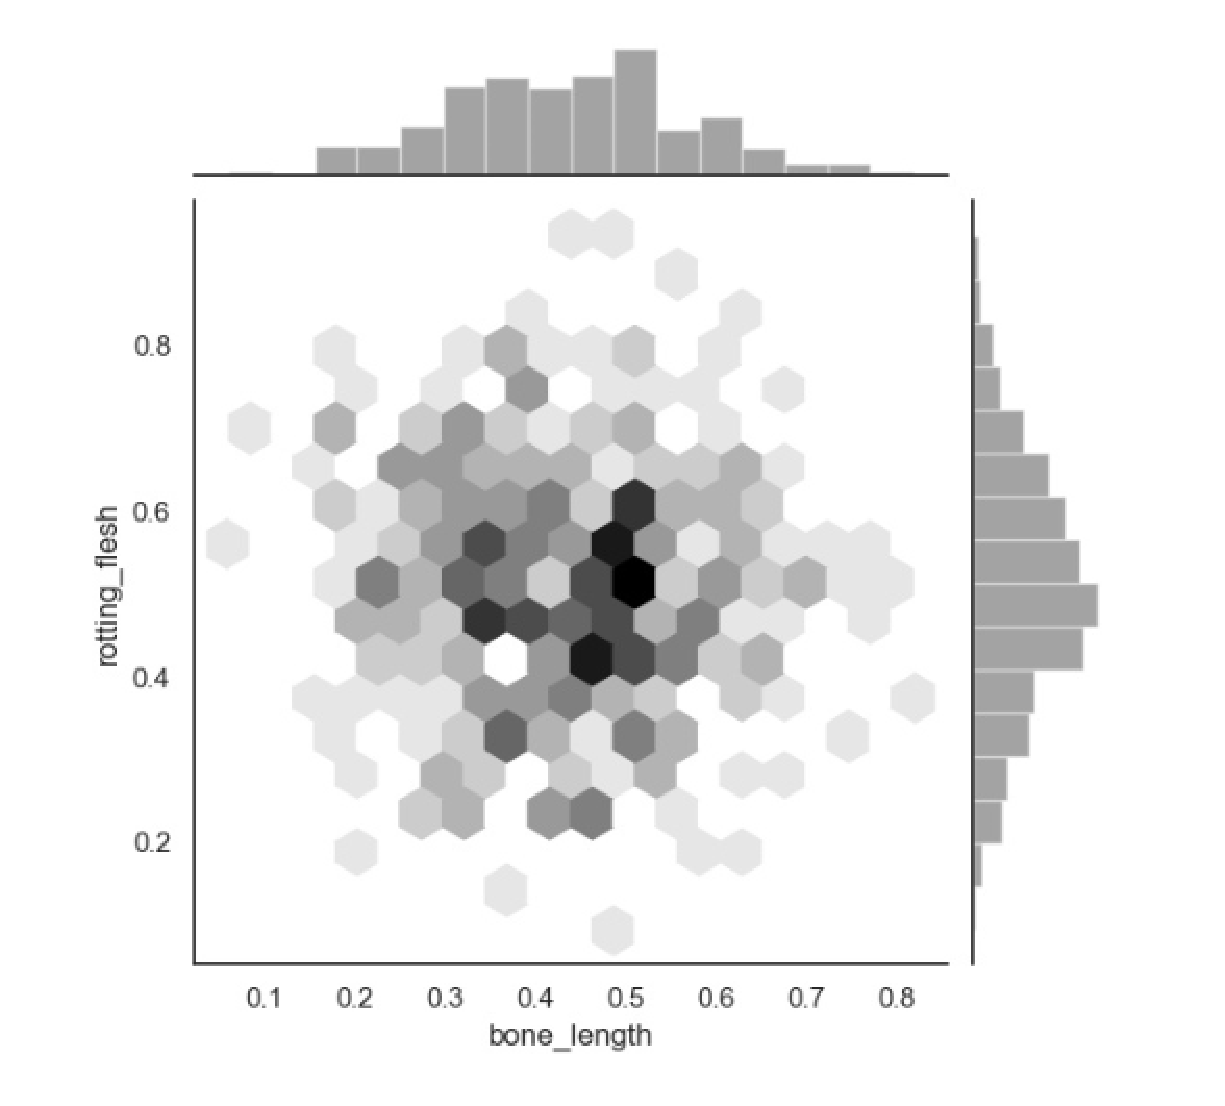
\includegraphics[scale=0.3]{figures/MHis.eps}
	\caption{Marginal Histogram}
\end{figure}

\begin{figure}[h]\centering
	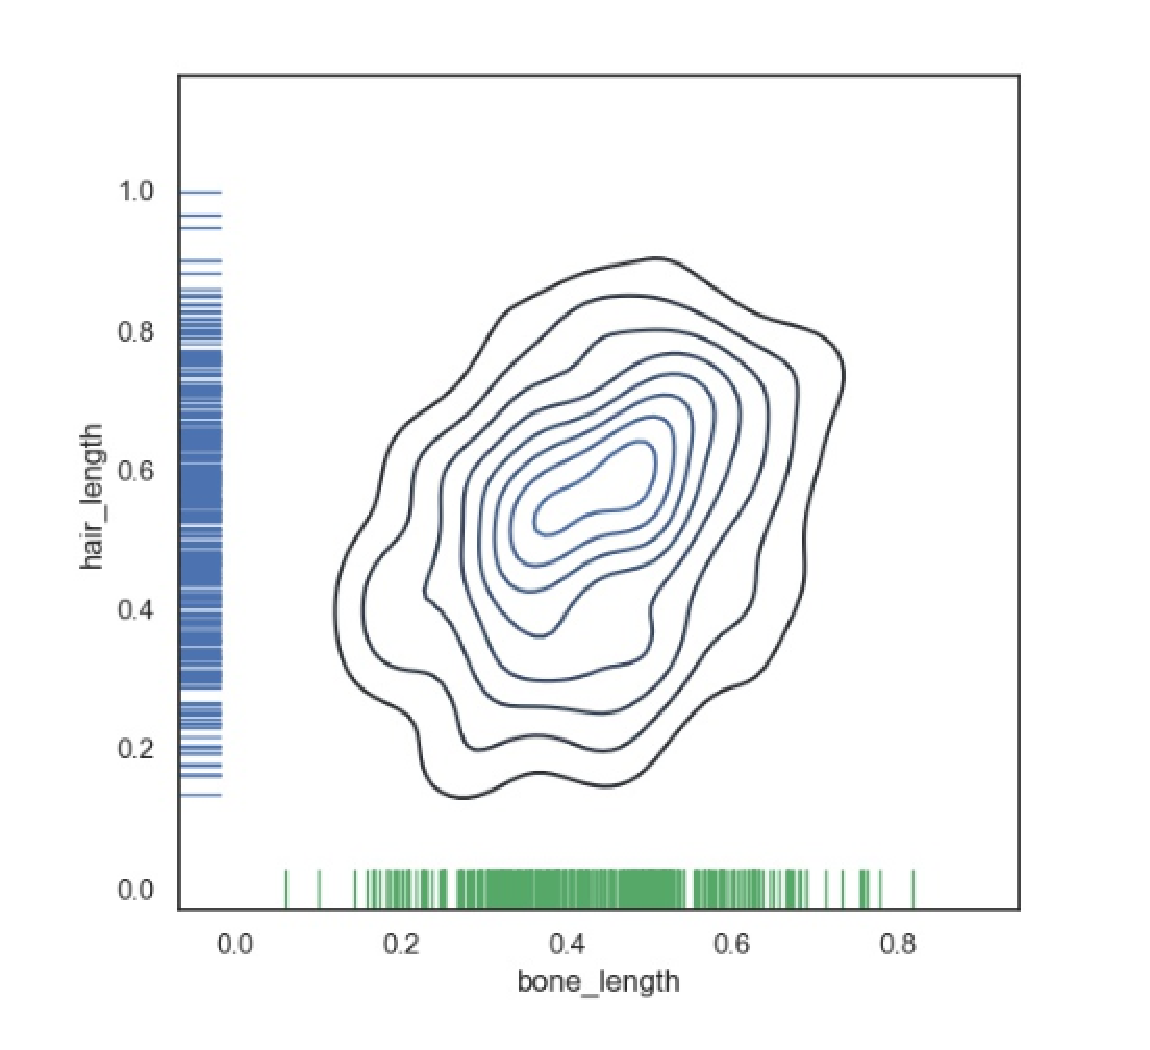
\includegraphics[scale=0.3]{figures/BDF.eps}
	\caption{Binary Density Function}
\end{figure}

\begin{figure}[h]\centering
	%\graphicspath{{figures/}{mine/}}
	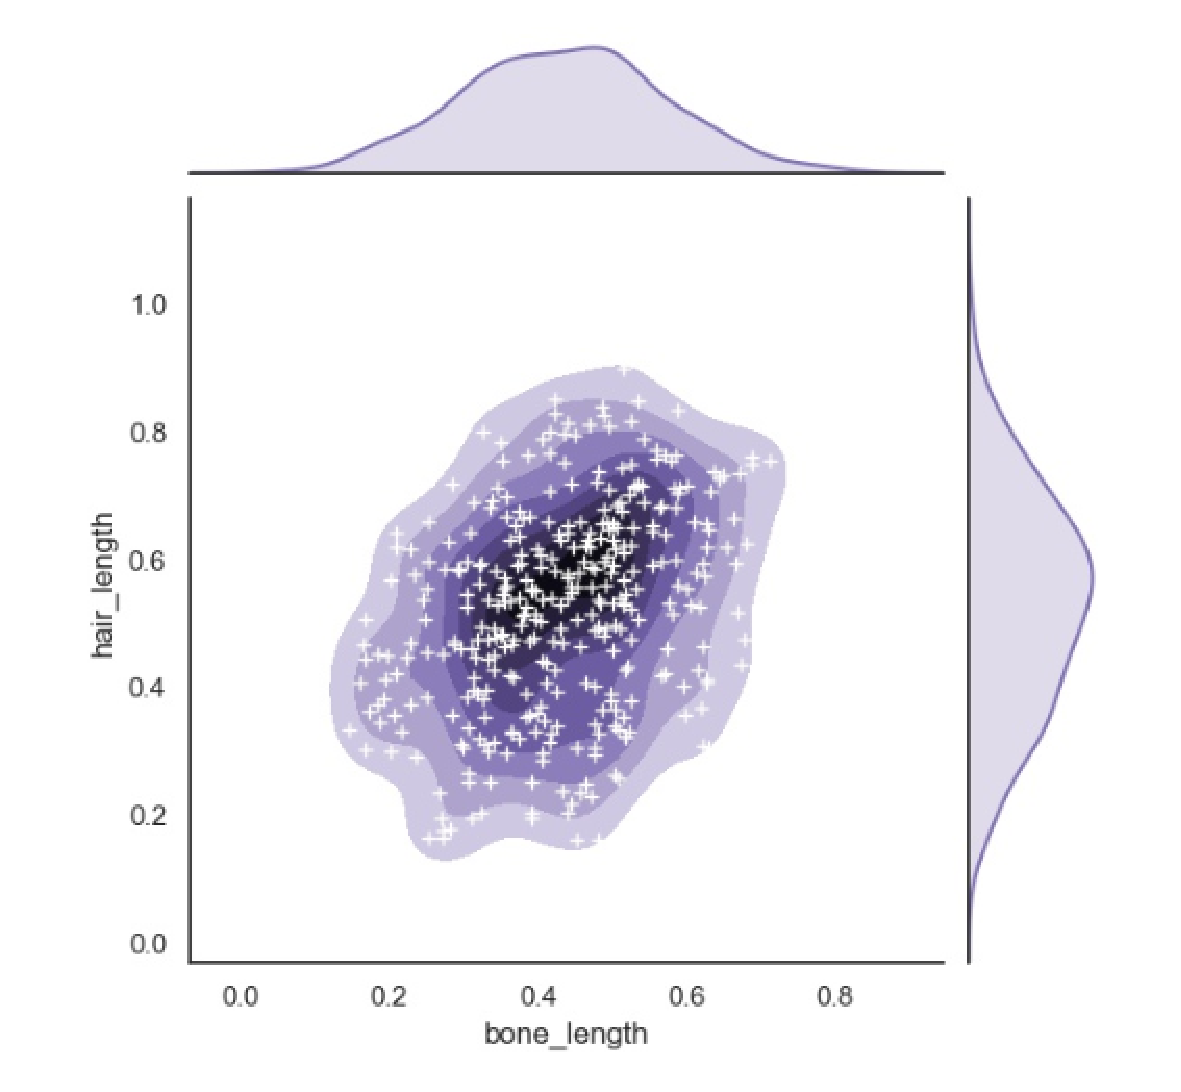
\includegraphics[scale=0.3]{figures/MBDF.eps}
	\caption{Marginal Binary Density Function}
\end{figure}


\subsection{Data Preparation}

\subsubsection{Great New Features}


As it can be seen from 
the pictures above 
the data is distributed normally. 
But some of them show clusters: 
hair_length and has_soul, 
hair_length and bone_length. 
So create new variables 
with multiplication of these columns: 

\begin{description}
	\item[hair_soul] row[’hair_length’]*row[’has_soul’] 
	\item[hair_bone]  row[hair_length]*row[bone_length] 
	\item[bone_soul]  row[bone_length]*row[has_soul] 
	\item[hair_soul_bone]  row[hair_length]*row[has_soul]*row[bone_length] 
\end{description}


Then analyse the new features in a pairplot, 
showing the picture ~\Cref{fig:new_pairplot}
below. 
It can be seen from the picture that 
there is a clear linear relationship 
between the variables. 


\begin{figure}[htbp]
	\centering
	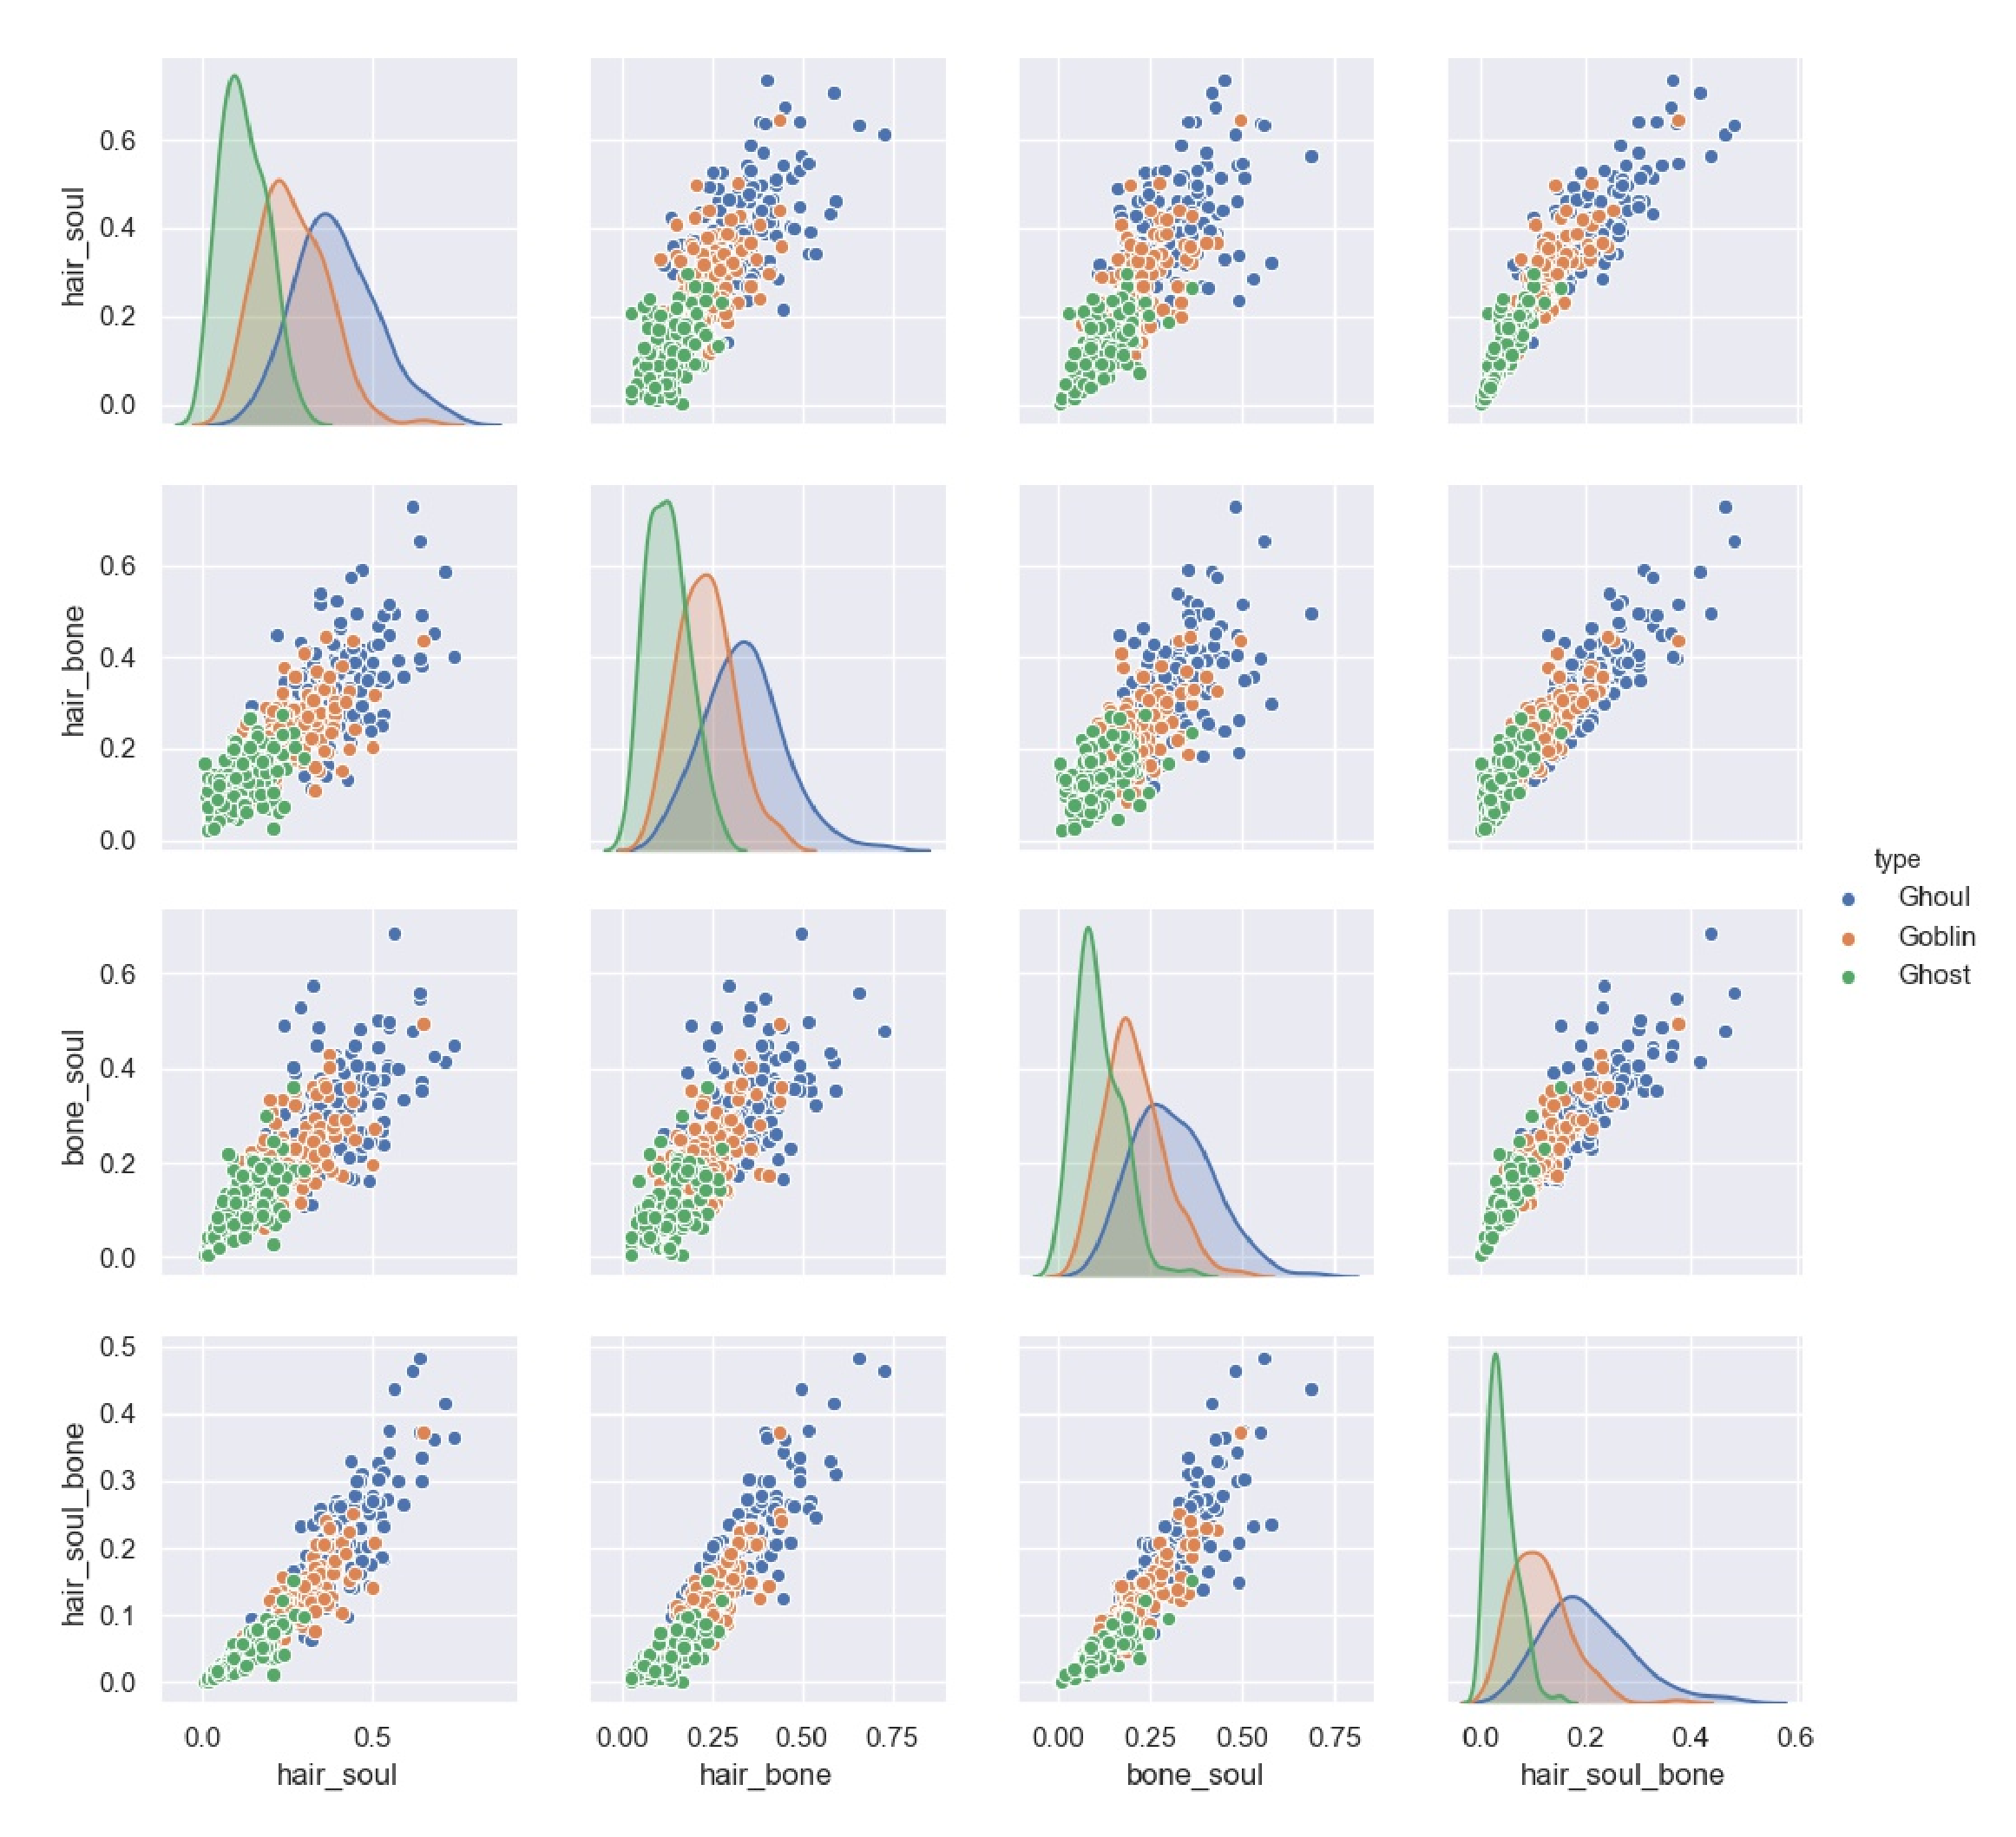
\includegraphics[scale=0.3]{figures/hist_1.eps}
	\caption{New Features Pairplot}\label{fig:new_pairplot}
\end{figure}


\subsubsection{Feature Selection}


Train Random Forest model first, 
then using the Feature Importance this function 
to select the most important features. 
The following figure ~\Cref{fig:feature_importance}
is a histogram ordered by feature importance. 


\begin{figure}[htbp]
	\centering
	%\graphicspath{{figures/}{mine/}}
	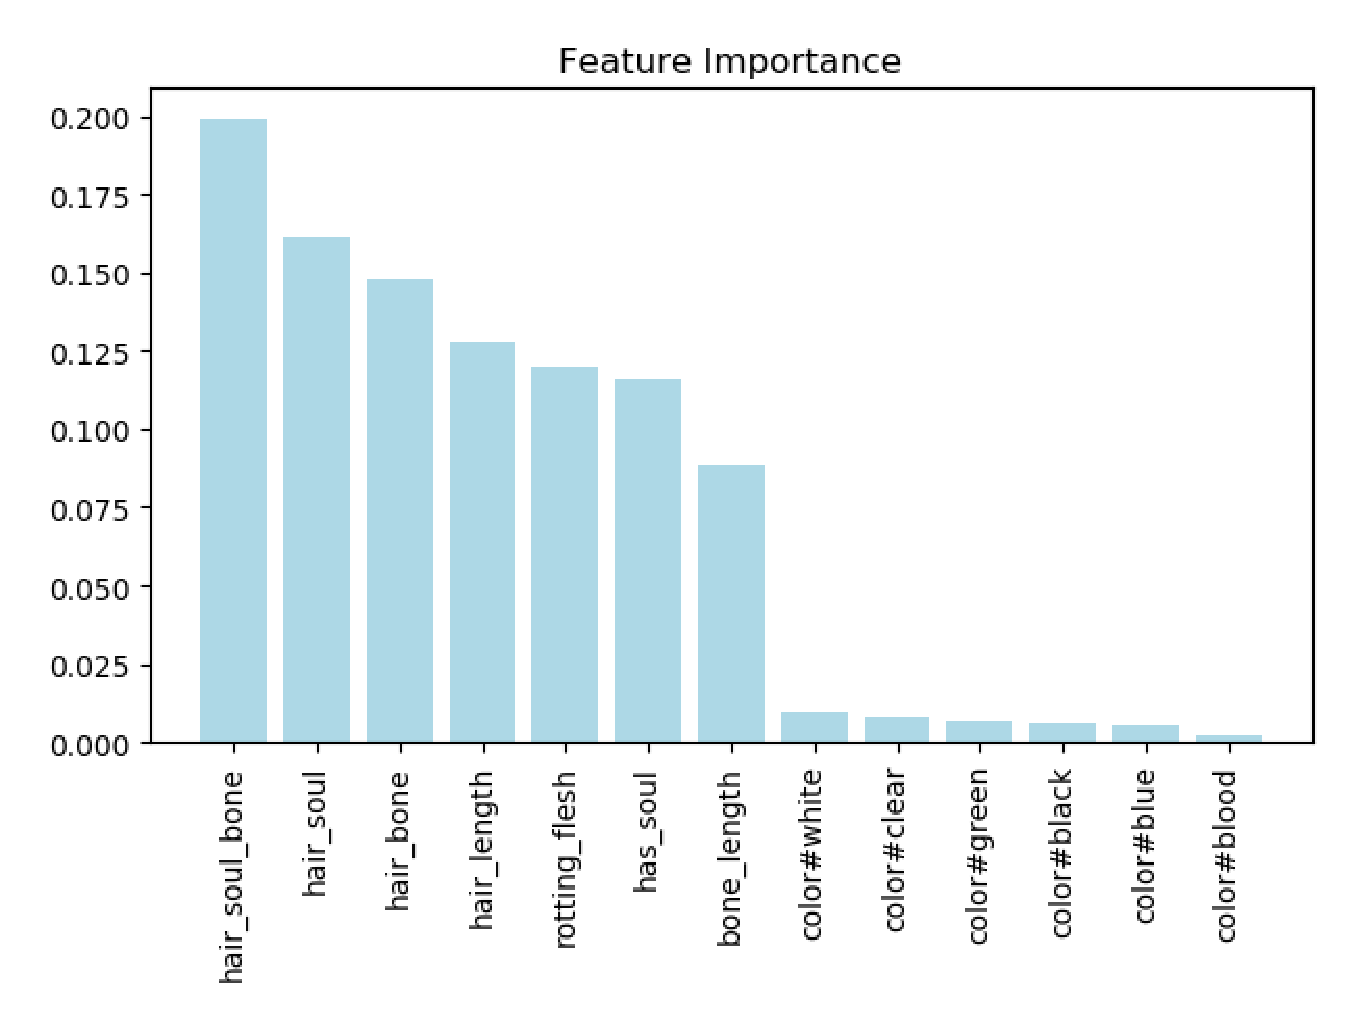
\includegraphics[scale=0.3]{figures/FEATURE.eps}
	\caption{Feature Importance}\label{fig:feature_importance}
\end{figure}

Take the top six features 
with higher importance 
to form a new train data.


\section{Method}

There are many machine learning algorithms 
for classification problem. 
Choose the following algorithms, 
explain the principles of
these algorithms and 
show the most important parameters.

\begin{itemize}
	\item RandomForest 
	\item Bagging
	\item GradientBoosting
	\item LogisticRegression
	\item SVC
	\item KNeighbors 
	\item XGB
	\item Netual Network
\end{itemize}

\subsection{RandomForest}


Random forest is a classifier with 
multiple decision trees, and
the output is determined by 
the mode of the individual tree output.

\begin{itemize}
	\item Principle
	
	\begin{itemize}
		\item Use M to indicate the number of training samples, 
		and N to indicate the number of features.
		\item The number of feature inputs n is 
		used to determine the decision result 
		of a node on the decision tree; 
		where n should be much smaller than N.
		\item From the M training samples, 
		the sampling is performed k times to 
		form a training set (ie bootstrap sampling), 
		and the unused use cases (samples) are 
		used for prediction to evaluate the error.
		\item For each node, 
		n features are randomly selected, 
		and the decision of each node on each decision tree is 
		determined based on these characteristics. 
		According to these n features, 
		calculate the best split mode.
		\item Finally, predict the test data and 
		decide the classification 
		according to each tree in a multi-winning manner.
	\end{itemize}
	
	\item Parameters
	
	\begin{description}
		\item[n_estimators] the number of decision trees
		\item[criteriom] criterion of choosing 
		the most appropriate node
		\item[max_depth] The maximum depth of the tree, 
		the default is None 
		\item[max_features] The feature that is divided 
		when selecting the optimal attribute 
		cannot exceed this value.
	\end{description}

\end{itemize}


\subsection{LogisticRegression}

Logistic regression is the algorithm that 
processing a large amount of 
observation data to 
obtain mathematical expressions 
that are in line with 
the internal laws of things

\begin{itemize}
	\item Principle
	
	\begin{description}
		\item[Hypothesis] $h(x)=W^{T} x+b$
		\item[Parameters] $ W$, $x$
	\end{description}
	
	\item Parameters
	
	\begin{description}
		\item[Penalty] Regular function
		\item[C] Regular coefficient
	\end{description}
	
\end{itemize}
%J=sum(logloss(f(xi), yi)) + C* penalty

\subsection{Bagging}


Bagging can improve the stability and accuracy 
of machine learning algorithms, 
it can reduce the variance of 
the model and avoid overfitting

\begin{itemize}
	\item Principle
	
	\begin{description}
		\item[INPUT] train data $ D = \left\{ 
		\left(x_1,y_1 \right), \left(x_2,y_2 \right),
		\dots,\left(x_m,y_m \right) \right\}$
		
		Base learning algorithm $L$
	
		Frequency of training $T$
		\item[OUTPUT] The best base learning algorithm $f(x)$
	
	\end{description}
	
	\item Parameters
	
	\begin{description}
		\item[n_estimators] Number of combined basic evaluators
		\item[max_samples] Number of basic estimator samples
	\end{description}
	
\end{itemize}

\subsection{GradientBoosting}

Gradient boosting uses gradient descend 
to find the best solvtion.
A major step in machine learning is 
to minimize the loss function $L(θ)$ 
by an optimization method to 
find the corresponding parameter $θ$. 
Gradient descent is 
a classic numerical optimization method.

\begin{itemize}
	\item Principle
	
	\begin{description}
		\item[Initialization] $ f_{0}(x)=	
		\operatorname{arg\,max}_\gamma 
		\sum\nolimits_{i=1}^n L(y_i,\gamma)$
		
		\item[for $m=1$ to $M$] 
		
		\begin{itemize}
			\item calculate negative gradient
			\item through minimizing the square error, 
			fitting the $ \tilde{y_i} $ 
			with the base learner $h_m(x)$
			\item use line search to 
			determine the step size $\rho_m$ to minimize $L$
		\end{itemize}
		
		\item[OUTPUT] $f_M(x)$
	\end{description}
	
	\item Parameters
	
	\begin{description}
		\item[learning_rate] control the speed of each update
		\item[n_estimators] he number of decision trees that 
		need to be used
		\item[max_depth] the maximum depth of the tree
	\end{description}
\end{itemize}
%\frac{\partial f}{\partial x} = 2\,\sqrt{a}\,x
\subsection{SVC}


The basic principle of the SVM algorithm is 
to find a hyper plane that can 
distinguish between two types, 
so that the margin is the largest.

\begin{itemize}
	\item Princible
	
	\begin{itemize}
		\item choose a kernel function, reduce the amount of calculation
		\item determining the hyperplane equation
		\item optimization model
	\end{itemize}

	\item Parameters
	
	\begin{description}
		\item[kernel] kernel function
		\item[C] penalty factor for error terms
		\item[degree] order of polynomial kernel function
	\end{description}
	
\end{itemize}

\subsection{KNeighbors}

The meaning of the knn algorithm is that 
enter new data without tags, 
compare each feature of the new data with 
each feature in the training set, 
and select the classification tag with 
the most similar feature (nearest neighbor: k)

\begin{itemize}
	\item Princible
	\begin{itemize}
		\item calculate the Euler distance of 
		the new sample point in the sample space 
		from all training samples
		\item Sort the Euler distances and 
		find the nearest k points
		\item Classify statistics on k points to 
		see which type of points has 
		the most number. 
		This type is the type of 
		prediction for new samples.
	\end{itemize}
	
	\item Parameters
	\begin{description}
		\item[n_neighbors] number of neighbors to use 
		by default for kneighbors queries
		\item[leaf_size] leaf size passed to BallTree or KDTree
		\item[p] power parameter for choosing 
		the distance calculation formula
		\item[weights] used in prediction
		\item[algorithm] compute the nearest neighbors
	\end{description}
	
\end{itemize}

\subsection{XGBoost}
 
XGBoost is to establish K regression trees 
so that the predicted value of 
the tree group is as close as possible to 
the true value (accuracy) and 
has the greatest generalization ability. 
From a mathematical point of view, 
this is a functional optimization, multi-target.

\begin{itemize}
	\item Princible
	\begin{description}
		\item[predictive model] $\hat{y_i}=\sum\nolimits_{k=1}^K f_k(x_i)$
		$K$ is the number of trees,
		$f_k$ represents the kth tree,
		$\hat{y_i}$ is the predictive result of $x_i$
		\item[loss function] $Obj(\theta)=\sum\nolimits_{i=1}^n l(y_i,\hat{y_i})+
		\sum\nolimits_{k=1}^K \Omega(f_k)$
		$l(y_i,\hat{y_i}$ is the train error of example 
		$x-i$, $\Omega(f_k)$ is the regular item of the kth tree.
	\end{description}
	
	\item Parameters
	\begin{description}
		\item[learning_rate]  control the speed of each update
		\item[n_estimators] number of iterations
		\item[max_depth] the depth of tree
		\item[gamma] penalty factor%惩罚系数
		\item[subsample] the proportion of data used in 
		all training sets when training each tree
		\item[colsample_bytree] the proportion of features used 
		in all trees when training each tree
	\end{description}
\end{itemize} 

\subsection{Netual Network}




\subsection{Ensemble Model}
There are many machine learning algorithms, 
select the following machine learning algorithms as Ensemble Model’s base models. 


\section{Experiment and Result}

\subsection{Model Training}
meters,but the more important ones are generally not too many. Determine a set of optimal parameters through Grid Search. Because the training data is relatively small, a ten-fold cross-validation is used. %



\subsection{Ensemble Model Training Result}

The results of using Grid Search to find the optimal parameters and the best accuracy of the algorithm are as 
 
follows. The best score is the score which is best in ten-fold cross-validation, best parameters is the 

parameters of the algorithms that can gain the best score, and the accuracy score is the accuracy of the 

algorithms on the test data. 

\subsubsection[Train_Data_1]{Use the all attribute value}

\begin{itemize}
	\item Best Parameters of the Base Models
	
	\begin{itemize}
		\item RandomForestClassifier
		
		\begin{description}
			\item[Best Parameters] 'criterion': 'entropy', 'max_depth': 5, 'max_features': None, 'n_estimators': 100
		\end{description}
		
		\item BaggingClassifier
		
		\begin{description}
			\item[Best Parameters] 'max_samples': 10, 'n_estimators': 100 'n_estimators': 100
		\end{description}
		
		\item GradientBoostingClassifier
		
		\begin{description}
			\item[Best Parameters] 'learning_rate': 0.3, 'max_depth': 2, 'n_estimators': 20
		\end{description}
		
		\item LogisticRegression
		
		\begin{description}
			\item[Best Parameters] 'C': 1, 'penalty': 'l1'
		\end{description}
		
		\item SVC
		
		\begin{description}
			\item[Best Parameters] 'C': 10, 'degree': 3, 'kernel': 'linear'
		\end{description}
		
		\item KNeighborsClassifier
		
		\begin{description}
			\item[Best Parameters] 'algorithm': 'auto', 'leaf_size': 10, 'n_neighbors': 20, 'p': 5, 'weights': 'uniform'
		\end{description}
		
	\end{itemize}
		
	
	\item Best Score of the Base Models
	
	\begin{table}[h]  \centering
		\caption{Best Score of the Base Models}
		\label{tbl:best_score}
		\begin{tabular}{ccccccc}
			\hline
			% after \\: \hline or \cline{col1-col2} \cline{col3-col4} ...
			Base Models& RandomForest & Bagging & Boosting & LogisticRegression & SVC & KNN \\
			\hline
			Best Score & 0.7143 & 0.7305 & 0.7358 & 0.7332 & 0.7385 & 0.7088 \\
			\hline 
			%\bottomrule
		\end{tabular}
	\end{table}
		
	
	\item Metrics Classification Report of Ensemble Model
	
	\begin{table}[h]  \centering
		\caption{Metrics Classification Report of Ensemble Model}
		\label{tbl:metrics_classification_ensemble}
		\begin{tabular}{ccccc}
			\hline
			& precision  &  recall & f1-score &  support\\
			\hline
			Ghost   &    0.80   &   0.83  & 0.82 & 24\\
			Ghoul  &  0.88  &  0.79  &   0.84   &   29\\
			Goblin  &   0.67  &  0.73 &  0.70  &   22\\
			\hline
			micro avg  &  0.79  &  0.79  & 0.79    &  75\\
			macro avg  &  0.78  & 0.78  &  0.78  &  75\\
			weighted avg  &   0.79  &  0.79 &  0.79  &  75\\
			\hline 
			%\bottomrule
		\end{tabular}
	\end{table}
	
	
\end{itemize}


\begin{itemize}
	\item RandomForestClassifier
	
	\begin{description}
		\item[Best Score] 0.7142857142857143
		\item[Best Parameters] 'criterion': 'entropy', 'max_depth': 5, 'max_features': None, 'n_estimators': 100
		\item[Accuracy Score] 0.8133333333333334
	\end{description}
	
	\item BaggingClassifier
	
	\begin{description}
		\item[Best Score] 0.7304582210242587
		\item[Best Parameters] 'max_samples': 10, 'n_estimators': 100 'n_estimators': 100
		\item[Accuracy Score] 0.68
	\end{description}
	
	\item GradientBoostingClassifier
	
	\begin{description}
		\item[Best Score] 0.7358490566037735
		\item[Best Parameters] 'learning_rate': 0.3, 'max_depth': 2, 'n_estimators': 20
		\item[Accuracy Score] 0.88
	\end{description}
	
	\item LogisticRegression
	
	\begin{description}
		\item[Best Score] 0.7331536388140162
		\item[Best Parameters] 'C': 1, 'penalty': 'l1'
		\item[Accuracy Score] 0.76
	\end{description}
	
	\item SVC
	
	\begin{description}
		\item[Best Score] 0.738544474393531
		\item[Best Parameters] 'C': 10, 'degree': 3, 'kernel': 'linear'
		\item[Accuracy Score] 0.7466666666666667
	\end{description}
	
	\item KNeighborsClassifier
	
	\begin{description}
		\item[Best Score] 0.7088948787061995
		\item[Best Parameters] 'algorithm': 'auto', 'leaf_size': 10, 'n_neighbors': 20, 'p': 5, 'weights': 'uniform'
		\item[Accuracy Score] 0.7333333333333333
	\end{description}
	%\item XGBClassifier
\end{itemize}
 




%\lstset{language=python}         
%\begin{lstlisting}[frame=single]  % Start your code-block
%rf = RandomForestClassifier(random_state = 0)
%clf = GridSearchCV(rf, param_grid = params, scoring = accuracy_scorer, cv = 10, n_jobs = -1)
%clf.fit(X_train, y_train)
%y_pred = clf.predict(X_test)
%\end{lstlisting}



Parallel Coordinates 
Parallel coordinates helps to visualize if a feature helps to segregate the groups effectively. If a segregation is effected, that feature is likely going to be very useful in predicting that group.
%Analyzing the correlation between other features it's possible to see that 'has_soul' and 'hair_length' have an interesting value as well as the column 'has_soul' with 'rotting_flesh'. Lets then try to extract some new features from here. 
%Test citation~\cite{BL12J01}. 
%\begin{JournalOnly}
%and~\citep{BJL11J01} or~\citet{BJL11J01}.
%\end{JournalOnly}

%This is for~\cref{tbl:overall-experiments}, 
%\todo[fancyline]{Testing.}
%and this is for~\cref{sec-conclusions}.
%\todo[noline]{A note with no line back to the text.}%
%\gangli{This is comment from Gang.}
%\qwu{Response from QW}

Number:
\num{123}.
\numlist{10;30;50;70},
\numrange{10}{30},
\SIlist{10;30;45}{\metre},
and
\SI{10}{\percent}

\missingfigure[figcolor=white]{Testing figcolor}


\begin{ConferenceOnly}
We have \SI{10}{\hertz},
\si{\kilogram\metre\per\second},
the range: \SIrange{10}{100}{\hertz}.
$\nicefrac[]{1}{2}$.

\missingfigure{Make a sketch of the structure of a trebuchet.}

\end{ConferenceOnly}


For~\cref{eq:test},
as shown below:

\begin{equation}\label{eq:test}
a = b \times \sqrt{ab}
\end{equation}

\blindmathpaper

\section{Preliminaries} \label{sec-preliminaries}

\blindtext

\gliMarker  %TODO: GLi Here


\section{Method} \label{sec-method}

\blindtext
\blindlist{itemize}[3]
\blinditemize
\blindenumerate

\blindmathtrue
\blindmathfalse
\blinddescription


\section{Experiment and Analysis} \label{sec-experiment}


\begin{table}  \centering
  \caption{Precision Comparison on Event Detection Methods}
  \label{tbl:overall-experiments}
  \begin{tabular}{cccc}
\toprule
    % after \\: \hline or \cline{col1-col2} \cline{col3-col4} ...
    & OR Event Detection & AC Event Detection & TC Event Detection \\
\midrule
    precision & 0.83 & 0.69 & 0.46 \\
    recall & 0.68 & 0.48 & 0.36 \\
    F-score & 0.747 & 0.57 & 0.4 \\
\bottomrule
\end{tabular}
\end{table}


\section{Conclusions} \label{sec-conclusions}

\blindtext

\section*{Acknowledgment}

\lipsum[1]


The authors would like to thank \ldots

